\chapter{B2B Case Studies}
In this chapter, \gls{b2b} solutions that have previously been under scrutiny will be discussed. Firstly, two case studies Jepson, Lundin (2011)~\cite{jepson2009freemium} and B2B Sales and Marketing Plan For Limecraft, Kalle Lamminpää (2014)~\cite{lamminpaa2014b2b} will be reviewed, then two proven and successful freemium-based businesses will be under scrutiny. This is done in order to propose a better business model in Chapter 6
.
\section{Freemium for Large Enterprises by Jepson, Lundin (2011)}
This master's thesis concerns the viability of freemium as a business model in expensive and advanced solutions in an enterprise market, and revolves around the Swedish software development company Teleopti.

\subsection{About Teleopti}
Teleopti is a world leading company in delivering software solutions for strategic workforce management (WFM) and telecom expense management (TEM). Their product offering is twofold, consisting of Teleopti CCC for WFM and Teleopti Pro for TEM. As far as sales channels are concerned, their products are purchasable directly from them as well as from partner resellers throughout the world. A Workforce Management (WFM) product makes sure that appropriately skilled personnel is placed at the correct place at an correct time. WFM contains six core parts: forecasting, staffing, scheduling, operating, analysing and reporting, with the forecasting module being a main proponent given its function is to try to predict staffing needs at various times. These parts can be seen in Figure~\ref{fig:wfm}. Teleopti CCC is the focal point in this study, as the thesis by Jepson \& Lundin pertains to this particular product. The WFM service provided by Teleopti aims to to optimize the performance of contact centers, back offices, branches and retail stores by managing staffig needs according to the workload. The solution is also agent-centric meaning that the workforce members are able to access the service through smartphones or other mobile platforms, while being able to manually control scheduling, monitor staffing needs in real-time and self-administer working shifts.  

\begin{figure}[H]
    \centering
    \fbox{\includegraphics[width=\textwidth]{figs/WFM.png}}
    \caption{The circular WFM process}
    \label{fig:wfm}
\end{figure}

Teleopti's CCC product has a modular design and features a basic package and a number of additional modules available for purchase. The basic package contains the modules Forecast, People, Shifts, Schedules, Intraday, MyTime and Reports. The Forecasts module predicts workload, Shifts optimises the schedule from predicted workload generated by the Forecasts module, People manages staff, Intraday monitors workload in real-time and takes action should workload exceed a certain threshold. Reports generates logs, enabling an evaluation of operations and MyTime is used by staff to view reports and schedules. Optional modules include Performance Manager for a more advanced Reports module, Real Time Adherence for monitoring staff in real-time, Payroll Integration for salary management and Employee Self Service, an employee tool for messaging and shift planning. The main building blocks of Teleopti CCC can be seen in Figure~\ref{fig:teleopticcc}.

\begin{figure}[H]
    \centering
    \fbox{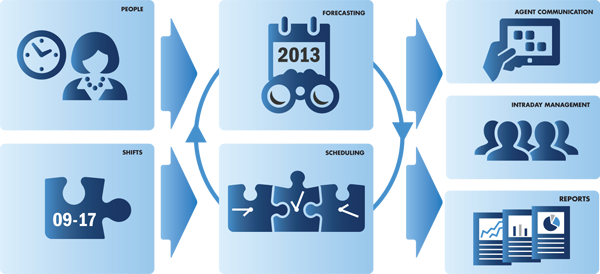
\includegraphics[width=\textwidth]{figs/teleopticcc.png}}
    \caption{Teleopti CCC's core functionality~\cite{teleopti2016}}
    \label{fig:teleopticcc}
\end{figure}

\subsection{Results}
Teleopti already has an established and premium product in Teleopti CCC, and with it being modular in design a module could be selected as being the focal point in generating leads in transitioning to a freemium model. Reasons for selecting just one particular module for giving away for free included modularity, creating demand for premium parts of the product and less adjustments needed to be made. Their recommendation fell on the Forecasts module as its features was possible to be used in isolation. Furthermore, this module was seen as a high-intensity feature of the product, as well as being a cornerstone in any WFM solution. It was further speculated that this module itself would generate the most demand for additional modules. A potential downside in choosing this model was the requirement of data from external sources.


Several points were made to make demand for the premium parts of the product, and as such it was suggested that additional paid features were left in the software, but greyed out leaving some of the features visible but not usable. However, technical limitations made this impossible and these additional modules were instead featured on the Teleopti Help webpage. In an effort to create as low entry barriers as possible, it was the decided that the best course of action was to simply require registration from users of the product. An emphasis was put on leads generation as a main proponent of a freemium model, and as such contact information from the free users was deemed necessary in order to raise demand for the premium parts of the product. Manual authorisation of new customers of the free part was suggested, as having documentation and instruction only available to authorised users making it harder for competitors to gain a competitive advantage on Teleopti as well as bringing a feeling of exclusiveness to its users.


It was pointed out that thorough documentation needed to be in place in a freemium product, to make sure new users adopt to the product and to minimise support costs. Comprehensive documentation of different levels of user proficiency was therefore suggested, to minimise support costs for the Teleopti support team. Having a larger user base as a result of freemium would also lead to more bug discoveries and fixes, easily remedied by patching the product for premium and free users alike. This can be seen as a positive externality as a result of an increased customer base using a freemium business model. 


Marketing Teleopti's brand and product were viewed as key success factors. The two main goals of launching a freemium product were to increase leads generation (thusly accelerating customer acquisition) and to raise awareness around Teleopti's brand. It was pointed out that Teleopti wished to state clear intentions when gaining new customers, in that their goal was to eventually sell their premium product, as having a hidden agenda may prove to have adverse effects in a \gls{b2b} setting. It was deemed important that in all communications had a clear message of what they were selling, how much it cost and that the free product is a part of a larger software package. Given that \gls{b2b} marketing differs from \gls{b2c} marketing, it was suggested that the channels used for marketing include the Internet, newsletters, business partners and press releases. Since Teleopti's intentions on eventually selling their premium product it was deemed necessary to rigorously follow up on free customers. This was realised by sending out a questionnaire to and telemarketing the customers of the free product. 


In conclusion, several success factors were listed as being detrimental for a freemium model in a \gls{b2b} market:
\begin{itemize}
    \item \textbf{First-to-market: }More attention for the target market, through PR and word-of-mouth. 
    \item \textbf{Adequate marketing communication: }Make sure there is no gap between the target market of the free and premium product, given the lead-generating aspect of freemium. Use appropriate marketing channels. Stimulate partners to market the free product, and clearly convey the type of product offered.
    \item \textbf{Stimulating demand for the premium product: }Make users aware that premium features or products exists, aswell as the brand of the premium product while following up on potential leads among the free users. 
    \item \textbf{User-friendly processes and product: }Having a robust and informative website with a simple and straightforward registration and installation process. Easy to follow and comprehensive documentation to reduce support costs, with support being free of charge.
    \item \textbf{Self-serviced customer services: }No internal resources needed for using the free product among customers, and keeping the free and premium equivalents close in function to avoid high maintenance costs. 
\end{itemize}

\section{B2B Sales and Marketing Plan For Limecraft by Kalle Lamminpää (2014)}
Lamminpää's thesis revolves around the Belgian start-up company Limecraft, in the business of media production. Founded in 2010, it delivers a product called Flow; a cloud-based software allowing media producers to share and collaborate their productions with each other~\cite{lamminpaa2014b2b}. This is a new way of moving footage between different personnel as opposed to the traditional way of transferring physical media physically. 


According to the thesis, Limecraft surveyed the large market that is the media industry, and estimated that around 2.5 million professionals worked in this field worldwide. In its infancy, Limecraft marketed their Flow product in the \gls{sme} market, as a freemium service. Onwards they discovered new markets in universities that often handle huge amounts of video in digital lectures etc. As in Freemium for Large Enterprises by Jepson, Lundin (2011), a large emphasis is put on leads generation. In Limecraft's case this was done at a large scale at the  Marché International des Programmes de Télévision (MIPTV) event in France where media professionals meet annually. Other trade fairs are also cited as being valuable venues for leads generation, as well as having a orderly website with clearly stated goals. 


Limecraft's freemium model was also described in a different manner than Teleopti's in the previous section: A free product was offered upon registration with 2.5GB of media storage, with this being expandable by inviting new users to the product or by upgrading to a premium payment model. However, issues arose when this particular model allowed for perpetual expansion of storage space and was consequently changed to a hard limit in volume of 5GB and only lasting three months. This is radically different from the freemium model proposed by Jepson \& Lundin (2011), and thusly the model offered by Limecraft can be viewed as being a trial version as opposed to freemium. A problem that followed was that the user-base didn't churn towards the premium product as expected. 


To remedy this several proposals were made by the Lamminpää: A larger social media presence, namely at Twitter, LinkedIn, through blogs and Slideshare, in order to be more visible on Google's search engine. Limecraft's sales cycle was reported at being around six months, making each customer more valuable. Freemium can possibly shorten the sales cycle~\cite{davidskokN/A}, but this is not mentioned by Kalle in this case. In conclusion, Lamminpää notes that a more aggressive marketing strategy should be employed, by empowering the social media presence of Limecraft, in addition to focusing on attending more trade conventions for leads generation. 


This particular case was included to demonstrate a company that has somewhat failed at employing the freemium model successfully, having reverted to a more traditional business model. This may be attributed to several factors including an inappropriate market for freemium products and Limecraft's reluctance in developing their product into the business paradigm that is freemium. 

\section{Successful B2B Freemium Ventures}
This section will review two services within the \gls{b2b} market that has successfully implemented a freemium model: Box and Splunk. These will be introduced in addition to listing possible success factors.
\subsection{Box}
\subsubsection{About}
Box was founded in 2005 by Aaron Levie and Dylan Smith, offering online file sharing and content management services for businesses. The free part of Box is limited to personal accounts for one users, with limits imposed on both storage and maximum file size. The premium side allows for enterprise and business accounts with potentially limitless storage options. Several users per account is also allowed, with better collaboration, administration and security features~\cite{freemium.orgN/A}. In 2010 they reported having a userbase of 10 million users divided amongst 120,000 businesses, with a free-to-premium churning rate of 8\%. Additionally, Box claims that 82\% of the largest companies in the world uses Box.
\subsubsection{Success factors}
Some of Box's success can be attributed to the ideas emerging from Box's leaders: They have stated that technical solutions are first and foremost used by its actual users, not management. This is reflected in their business model which only offers free Box accounts to non-enterprise entities, in the hope that that these users will act as proponents of Box's products in their respective businesses. Another important philosophy stated by Levin is the importance of keeping customers in a \gls{saas}-setting happy~\cite{tientzuozuora2014}\cite{youtube2011}. They believe happy customers are more willing to pay as long as a good product is in place to begin with, a prerequisite of the freemium business model. The use of the freemium model (albeit in an indirect way in a \gls{b2b} setting), allows for penetration in markets previously being thought of as unreachable. Furthermore it is pointed out that in a freemium paradigm, non-paying customers are not lost to competitors.


As a company that delivers \gls{saas} services, revenues has to be viewed in a different manner than traditional means, where \gls{arr} is a better metric. It is self-explanatory that in the long-term this can be more profitable, and this is shown in the Gross Recurring Margin for Box estimated at 79\% in 2014~\cite{tientzuozuora2014}. This shows that their costs are acceptable, and furthermore, their Recurring Revenue Margin (\gls{arr} minus sales, R\&D and G\&A costs) grew from 8\% in April of 2013 to 20\% in January of 2014. These facts combine may indicate that Box is an expanding and profitable business. Lastly, Box also has an \gls{api}, enabling users of Box to customise and integrate Box into existing systems, apps and services. Box also allows external innovation through their provided \gls{api}, making it possible for developers to make apps in the Box ecosystem and monetise these apps. 

\subsection{Splunk}
\subsubsection{About}
Splunk was founded in 2003 by Michael Baum, Erik Swan and Rob Das, and is a software company producing software for analysing, monitoring and searching big data~\cite{derrickharris2010}. Splunk offers their software either as a platform or \gls{saas}, and features these either as an Enterprise package or a Light package with the latter being aimed at smaller IT environments. The difference between these two lies in their respective premium packages: Light has a limit on daily data volume and maximum users, while Enterprise does not have this limitation. The rest of the differences are smaller in magnitude, but Enterprise customers can also access \glspl{api}, and enjoy more rigorous support. The \gls{saas} versions operate on a free trial basis with a limit on 5GB of cloud storage per day, while the platform versions have a limit of 500MB of indexed data per day. After 30 days of usage, the users of the platform-version may continue with a free license or upgrade to a premium version. Splunk's revenues were estimated to have increased by 50\% from 2015 to 2016, expecting annual revenues around 850 million USD. They have more than 10 000 customers across 100 countries and 1700 employees.

\begin{figure}[H]
    \centering
    \fbox{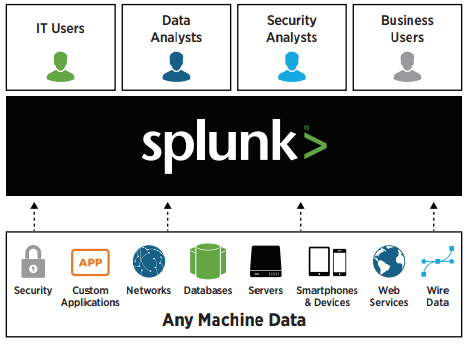
\includegraphics[width=\textwidth]{figs/splunk.PNG}}
    \caption{Splunk's Enterprise product~\cite{splunkinc20162}}
    \label{fig:splunk}
\end{figure}

\subsubsection{Success factors}
Initially, only the platform version of Splunk was offered but they later expanded to a subscription-based \gls{saas} offering, representing 37\% of revenues. Focus was also shifted towards enterprise customers as opposed to \gls{smb} customers, and they report that up to 70\% of customers convert their free licenses to premium ones, utilising the additional features the premium model allows~\cite{philiplay2014}. Much of Splunk's success also comes from providing a mission-crucial service in security and IT services, and focuses more and more on sales and customer support given its growth. The rich information and real-time analysis provided by Splunk enables its customers to avoid security threats, monitor customer preferences, launch new products faster and saving money in the process. One of Splunk's main value propositions is to provide its customers with usable, valuable and accessible big data, eliminating any inherent inefficiencies among the customers. 